\documentclass[conference,a4paper]{IEEEtran}
\IEEEoverridecommandlockouts
\usepackage{textcomp}
\usepackage{graphicx}
\usepackage{cite}
\usepackage{algorithm}
\usepackage{algpseudocode}
\usepackage{amsmath}
\usepackage{amsfonts}
\usepackage{color}
\usepackage[tableposition=top]{caption}
\usepackage{setspace}
\usepackage{epstopdf}
\usepackage{graphics}

\begin{document}
\title{Investigation over NOMA with SIC in single antenna scheme}

\author{
\authorblockN{Ming Jie Yang}\\
\authorblockA{
GICE, National Taiwan University\\
Taipei, R.O.C\\
R02942125@ntu.edu.tw\\
2014 May 9th}
}
%\IEEEspecialpapernotice{{\fontsize{12pt}{1em}\selectfont February 2014}}
\maketitle

% abstract
\begin{abstract}
% describe the project and objectives
The report shows progress on the project that explores non-orthogonal
multiple access (NOMA) with successive interference cancellation (SIC).
The short term objective of current phase is to build a simulation
framework and examine the performance gain with SIC technique. The
system is extended based on LTE architecture.

% brief the content in this report

% brief some result


\end{abstract}

% describe project motivation, objectives and related works in details
\section{Introduction}
\label{sec_introduction}
%\section{Introduction}
% u can reorganized some content herer
%
%The following provides a short summary of related information in these papers.
%There are two different analysis of non-orthogonal multiple access (NOMA) and successive interference cancellation (SIC). One analyzes SIC from original Shannon capacity and anther start from modulation scheme and packet error rate (PER). The analysis starting from Shannon capacity is mainly proposed from DOCOMO Japan~\cite{cite_docomo1, cite_docomo2, cite_docomo3}. Another one from the aspect of modulation and PER is proposed from Bell Lab~\cite{cite_bell1,cite_bell2}.
%

Briefly, by the previous effort in literature survey, we summarize related work
as follows.
In~\cite{cite_docomo1}, the authors compare the performance between orthogonal 
frequency-division multiple access (OFDMA) and NOMA. They in particular
investigate successive interference cancellation (SIC) and state that
SIC receivers should follow the rule that the optimal order for decoding
is in the order of the increasing $\frac{|h|^2}{N}$. An NOMA/Multiple-Input
Multiple-Output (MIMO) scheme is proposed to achieve further capacity gain.
In~\cite{cite_docomo2}, the authors investigate the enhancement of the
cell-edge user throughput by using SIC in  the cellular downlink. They
propose an optimization method that can balance the throughput of cell-edge
users and interior users. The work in~\cite{cite_docomo3} is the extension
of~\cite{cite_docomo2}, where the authors investigate the use of FFR and
weighted PF-based multi-user scheduling with SIC in the cellular downlink.
They show that NOMA can help achieve user fairness.
%
%The detailed description of related work from DOCOMO Japan will be given in Section~\ref{sec_phy} and Section~\ref{sec_mac}.
%

Related work in~\cite{cite_bell1} not only considers the ideal channel
capacity but also analyzes SIC performance with respect to modulation schemes
and packet error rate (PER). A resource allocation algorithm is proposed to
leverage the spatial gain and the simulation results show that
proposed algorithm using NOMA with SIC achieves more than 100 percent throughput
gain comparing OFDMA. In~\cite{cite_bell2}, the authors investigate SIC and
proposed an iterative SIC receiver architecture with combined pilot/date based
channel estimation for efficient decoding of NOMA signals. The simulation
results show iterative SIC receivers reach low PER with weak SNR under a
reasonable complexity.

%the authors analyze the iterative SIC receiver structure and present simulation results of their receiver structure with respect to PER.
%The simulation results are also given in the aspect of PER. %The detailed description is also in the following paragraphs.

%In order to compare two different analysis, the following paragraphs are divided into two sections for different topics (PHY layer and MAC layer). The PHY layer in Section~\ref{sec_phy} shows the NOMA/SIC from two different aspects: starting from Shannon capacity and starting from modulation/PER. The MAC layer in Section~\ref{sec_mac} discusses resource allocation and scheduling problems. We make a conclusion in Section~\ref{sec_conclusion} and describe our future direction in Section~\ref{sec_futureWork}. 

% ideal mathematical model explanation.
\section{system model}
\begin{figure}[t]
\begin{center}
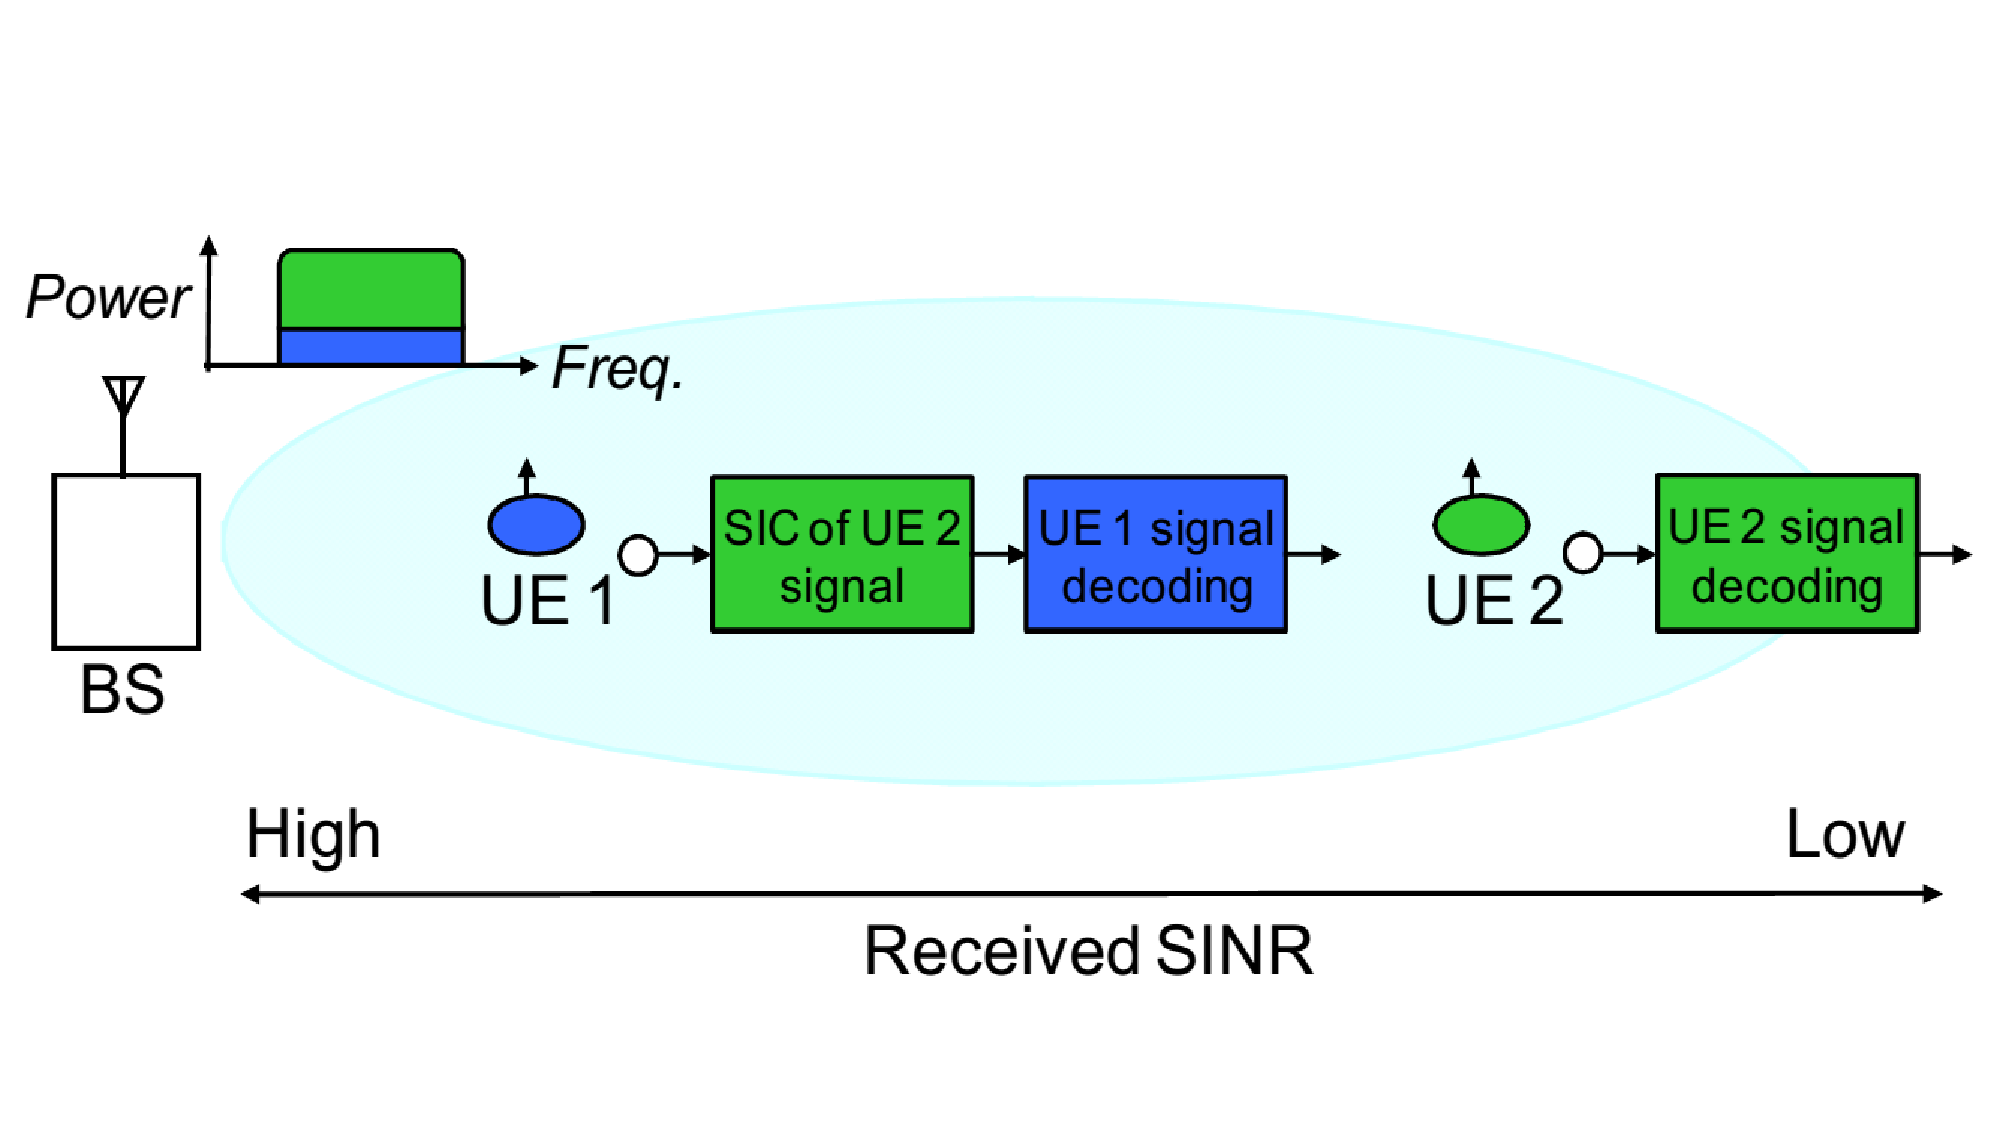
\includegraphics[width=1.0\columnwidth ,angle=0]{figure/NOMA_shannon}
\caption{Two-user SIC in the downlink}
\label{fig_NOMA_shannon}
\end{center}
\end{figure}
To understand how SIC works, take the two-user downlink communication in Fig.~\ref{fig_NOMA_shannon} as an example. The transmitted signal from the base station is a linear combination of the signals intended for UE1 and UE2. To decode individual signals, SIC needs to be performed at
each receiving UE. 
%In the NOMA downlink, the SIC process is implemented at the UE receiver. 
The optimal order for decoding is the order of the increasing channel gain normalized by the noise and inter-cell interference power. 
Assuming that the channel gain of UE1 is better than UE2, if UE2 can decode its signal, then UE1 must also be able to decode the UE2 signal.
Therefore, as shown in Fig.~\ref{fig_NOMA_shannon}, UE1 first decodes the signal of UE2 and then decodes its signal after the decoded
UE2 signal has been subtracted. 
%has to decode UE2's signal before decoding its signal, which is the concept of interference cancellation. 
For UE2, it can simply go ahead and decode its own signal without decoding the signal for UE1 first.
%However, UE2 does not perform interference cancellation. 
The case for SIC by $K$ UEs can be performed similarly, and ideally for any UE
the optimal decoding is to remove the interference coming from UEs with worse channel gains.
%, so (\ref{eq_sic_shannon}) is ideal interference cancellation.
As shown in~\cite{cite_docomo1}, 
the achievable rate $R_b^{\text{(sic)}}(k)$ for UE $k$ in resource $b$ can be represented as follows:
%accessing b-th resource and the k-th user throughput with SIC, , is represented as
\begin{equation}
\label{eq_sic_shannon}
R_b^{\text{(sic)}}(k)=W_b \text{log}_2 \left(1+\frac{|h_{k, b}|^2 P_{k, b}}{\displaystyle\sum^K_{{i=1} \atop {\frac{|h_{k, b}|^2}{N_{k, b}} < \frac{|h_{i, b}|^2}{N_{i, b}}}} |h_{k, b}|^2 P_{i, b} +W_b N_{k, b}} \right),
\end{equation}
where $|h_{i, b}|^2$ is channel gain between UE $i$ and the base station, $W_b$ is the bandwidth of resource $b$, $P_{i, b}$ is the transmission power allocated to UE $i$, and $N_{i, b}$ is the noise and inter-cell interference power for UE $i$.
% 分母中的sum是k沒有錯,指的是到第k-th user的i-th signal
Equation~\ref{eq_sic_shannon} shows a simple version of SIC reception model,
and the work in \cite{A_Successive_Interference_Cancellation_Scheme_for_an_OFDM_system}
investigate the design of a SISO SIC receiver operating on OFDM system
considering ICI cause by time variations in channel.
% fig
\begin{figure}[t]
\begin{center}
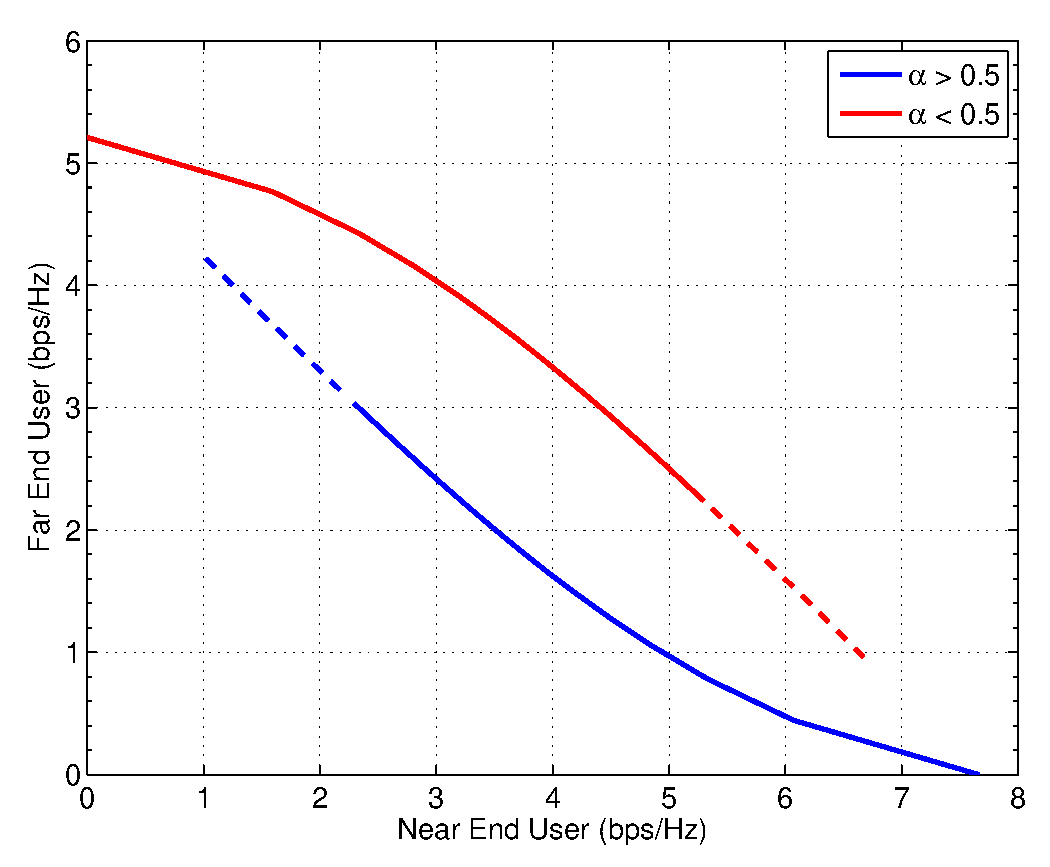
\includegraphics[width=0.95\columnwidth ,angle=0]{figure/u1VSu2.eps}
\caption{Upper boundary of rate in two users scheme}
\label{fig_ideal_r1r2}
\end{center}
\end{figure}
In the downlink scenario, the transmission power of the base station is limited
and denotes as $P$.
Assume there are two users that are served by the base station.
The power of the signal sent to near-end user, indexed as user 1, is $P_1=\alpha P$,
and far-end user, user 2, is $P_2=(1-\alpha)P$.
The channel is AWGN with pass loss exponent coefficient set to be $4.5$.
Consider the capture effect in receiving two signal in the same frequency, one with
stronger signal power will be demodulated. 
Thus as shown in Fig.~\ref{fig_ideal_r1r2}, when the power allocation factor $\alpha$
is greater than $0.5$, giving more power resource to near-end user, the curve is
convex. 
On the contrary, the curve is concave, which also indicates that there is
gain in weighted sum of throughputs.
The weighted sum rate \cite{cite_bell1} as a function of power allocation factor is 
defined as follows,
\begin{equation}
\label{eq_sic_weighted_sum_rate}
Gain = \frac{1}{R_1(P)}R_1(\alpha P) + \frac{1}{R_2(P)}R_2((1-\alpha)P)
\end{equation}
where $R_1$, $R_2$ are functions denotes channel capacity with given power allocated.
The measure for the system performance is enhanced by weighted sum rate, since optimizing
the sum rate of all users in the system results in serving specific user with good channel
condition.
% fig
\begin{figure}[t]
\begin{center}
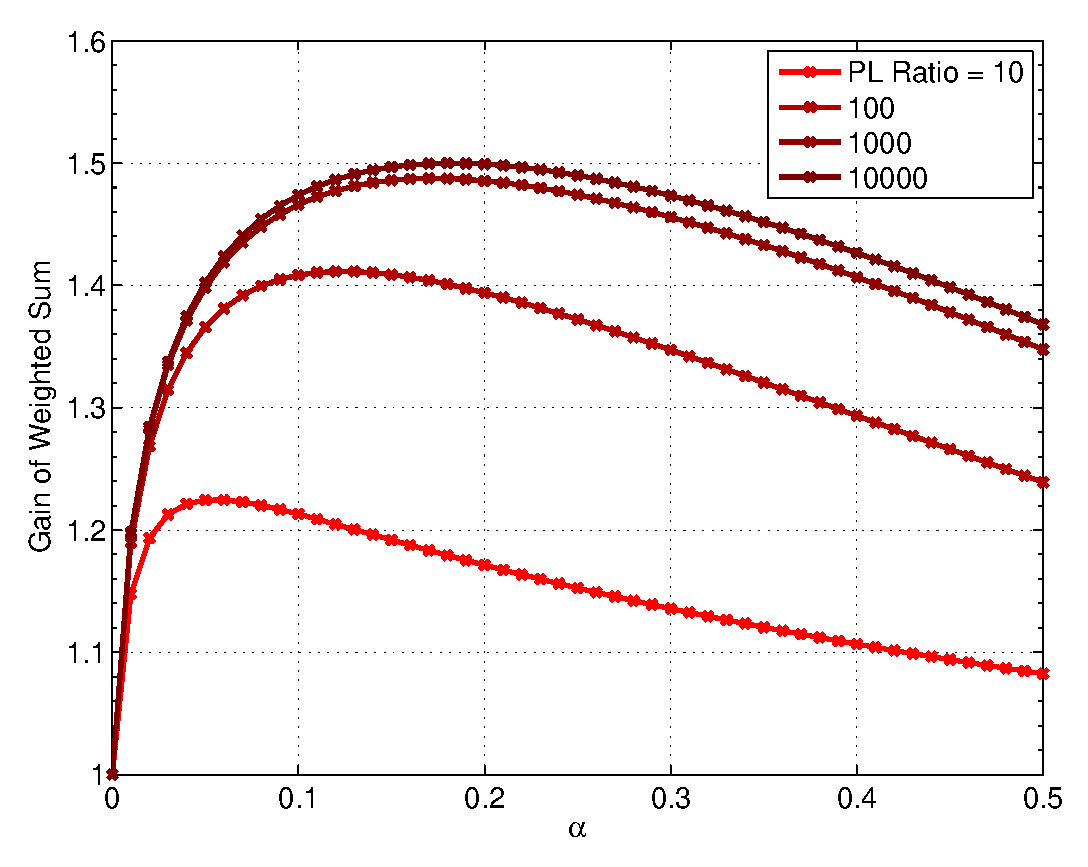
\includegraphics[width=1.0\columnwidth ,angle=0]{figure/alphaVSgain.eps}
\caption{Gain in Weighted sum of throughput for different PL ratio}
\label{fig_ideal_gain}
\end{center}
\end{figure}
In Fig.~\ref{fig_ideal_gain} the gain in weighed sum changes by different power allocation 
factor selected, and an optimal allocation varies for different pass loss ratio of user 1
and user 2.
As the difference of the PL ratio increase the gain in weighted sum increase also.
However, we've observed that the maximum of the gain is limited and possibly converges.


% simulations
\section{simulation}
To analyse how well the theoretical gains can be realized in practice, a more
sophisticated simulation is done to extend our investigation in NOMA with SIC.
The simulation is set up by following description.
\subsection{system architecture}
% fig
\begin{figure}[t]
\begin{center}
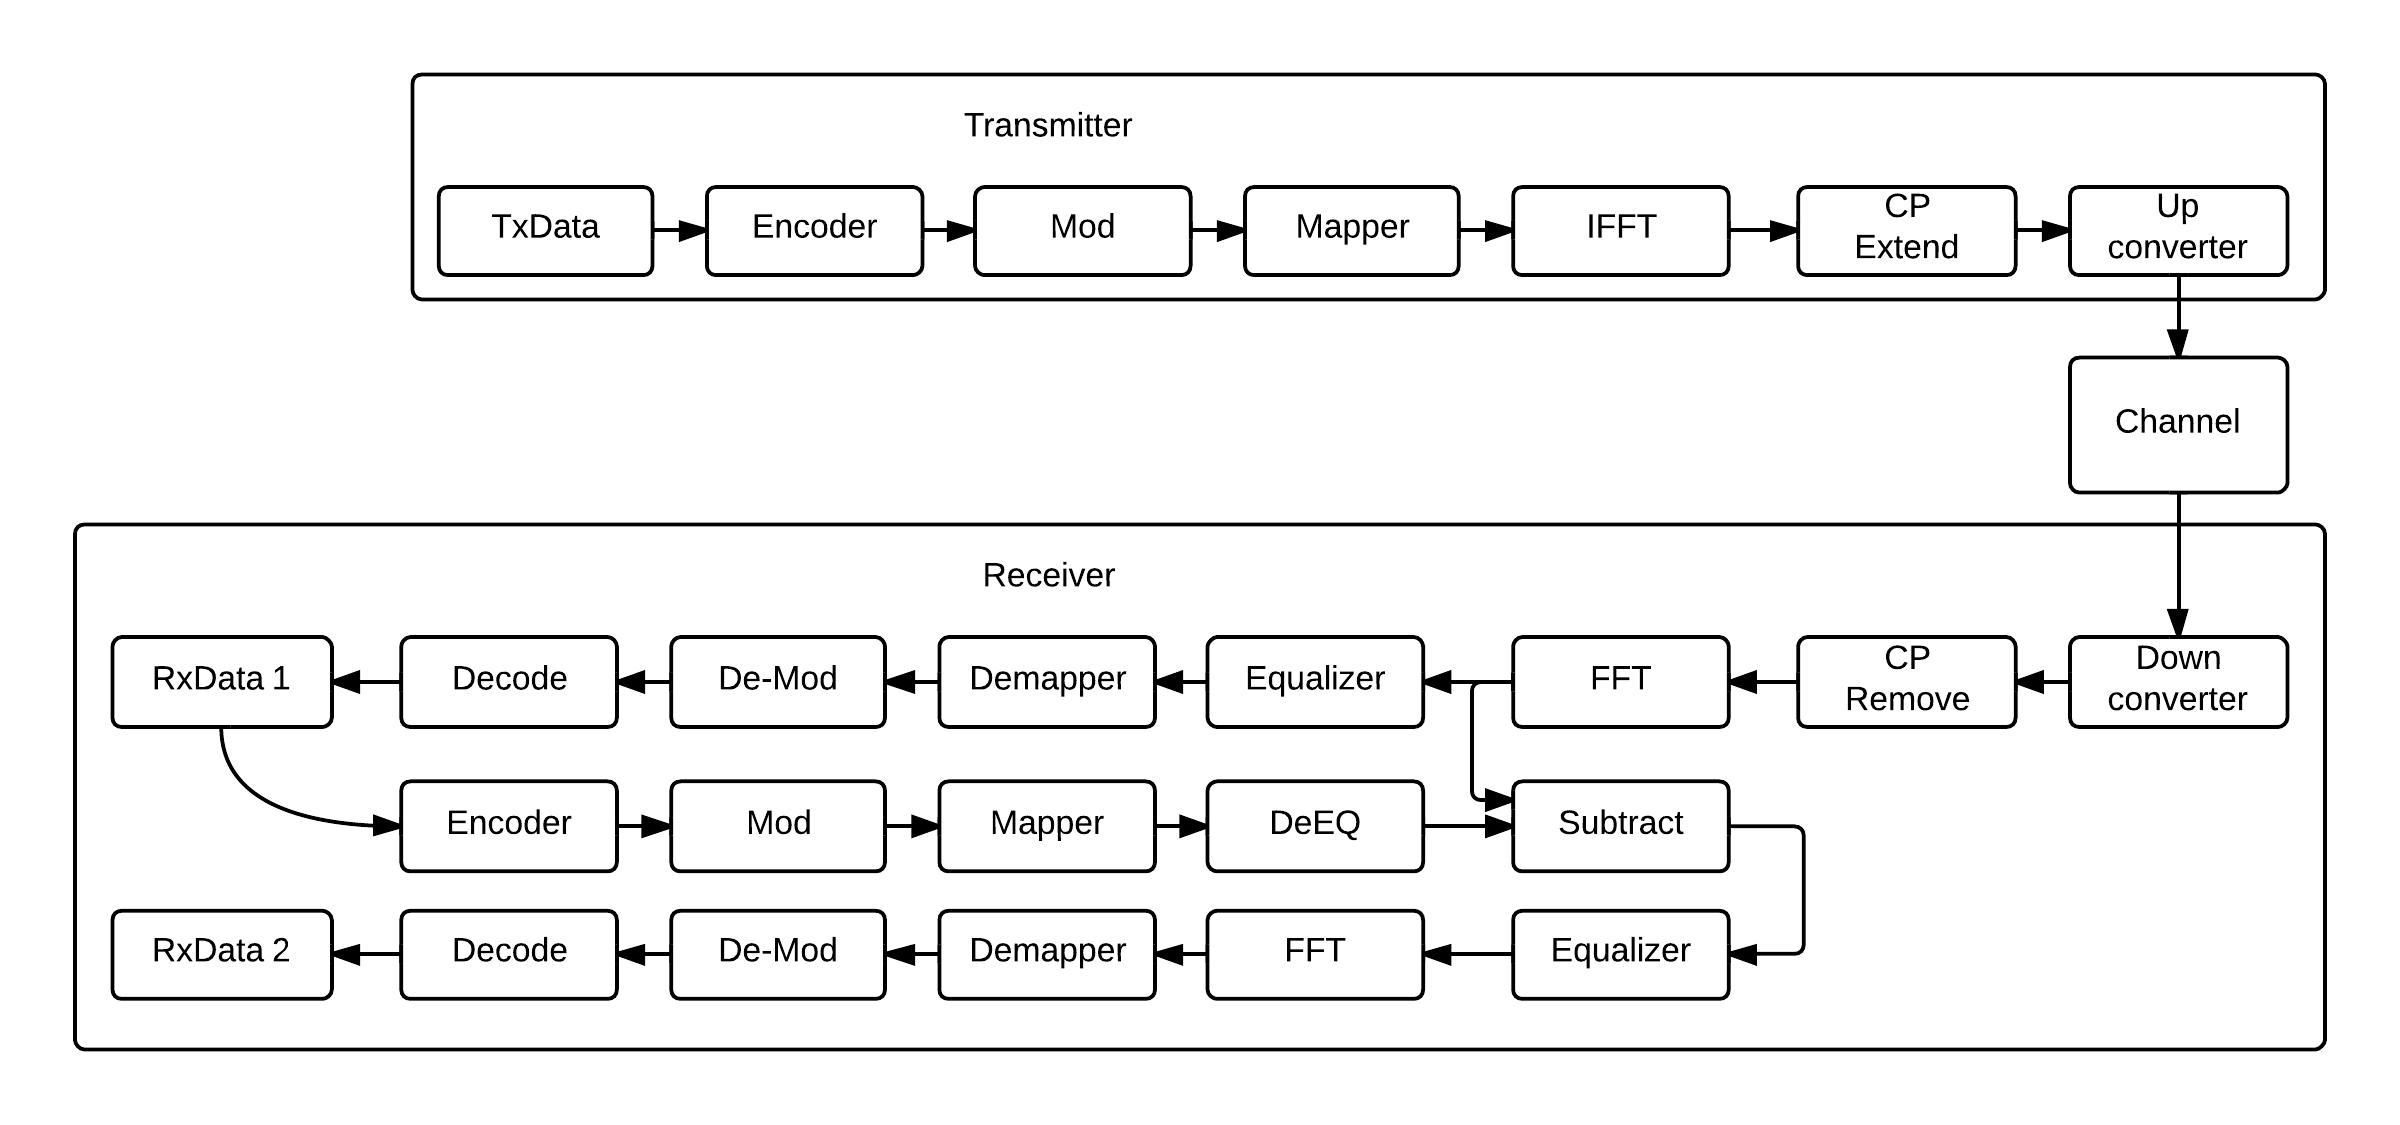
\includegraphics[width=0.95\columnwidth ,angle=0]{figure/systemArch.png}
\caption{Simulation system architecture block diagram}
\label{fig_sys_arch}
\end{center}
\end{figure}
The system architecture is shown in Fig.~\ref{fig_sys_arch}.
[Todo]
\begin{itemize}
  \item FFT size : $2048$
  \item Cyclic prefix length : $144$ samples
  \item Carrier frequency : $2.6$ GHz
  \item Bandwidth : 20MHz
  \item Modulation : BPSK, QPSK, 16QAM
  \item Coding rates : 
  \item Channel : AWGN, multipath fading channel
  \item Equalizer : MMSE
\end{itemize}
\subsection{numerical results}
In this section, extensive simulations are carried out to
examine the analytical results derived above.
$1M$ bits of data is transmitted in following simulations. 
\subsubsection{power allocation}
% fig
\begin{figure}[t]
\begin{center}
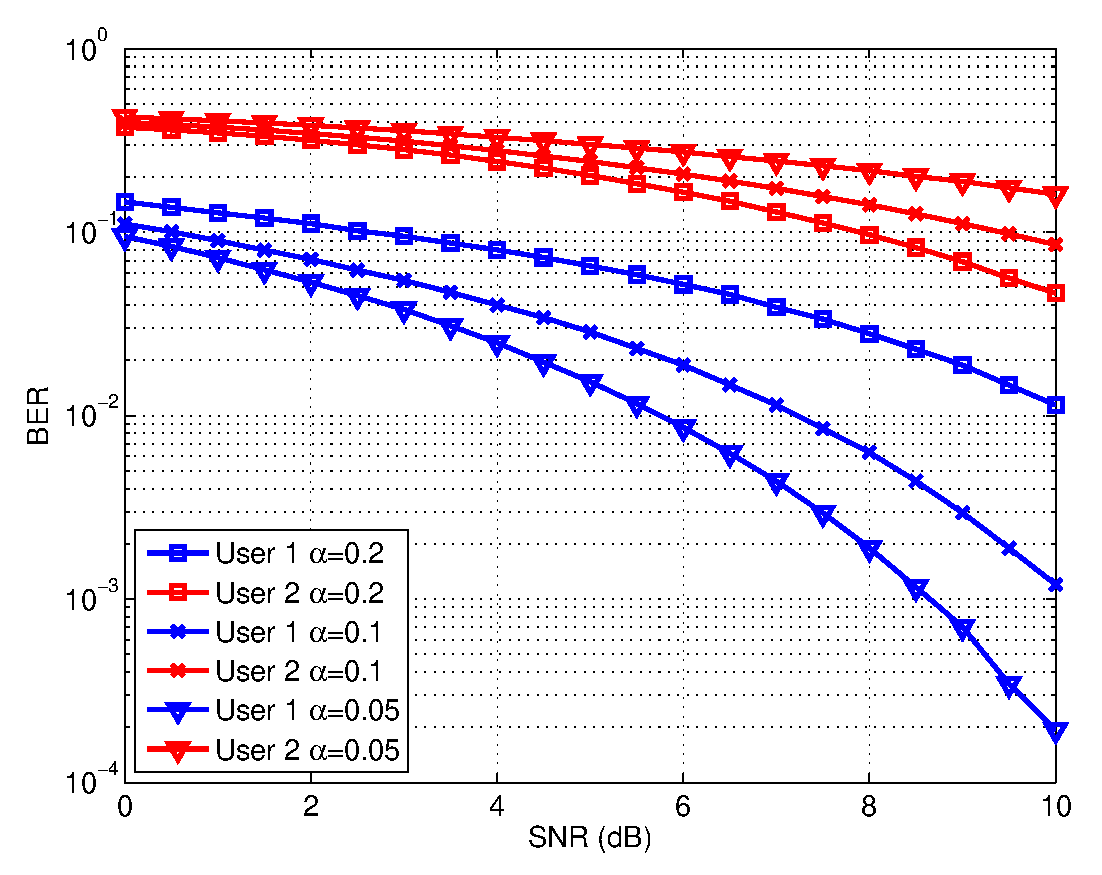
\includegraphics[width=0.95\columnwidth ,angle=0]{figure/snrVSber.eps}
\caption{BER performance of two users with identical channel condition}
\label{fig_sim_snrVSber}
\end{center}
\end{figure}
As in the previous mathematical model, whether or not the desired transmission
signal can be demodulated is not taken into account.
When the base station allocates similar power resources on both users' signals,
the receiver may not be able to extract any of the original data.
In other words, the region where alpha is set near 0.5 have to be checked.
Also, we would like to see the performance of SIC when user 1 and user 2 have
identical channel condition when served by the same base station.

In Fig.~\ref{fig_sim_snrVSber} shows BER curve for 2 users served in same BS 
with same channel condition.
The data stream is multiplexed by power allocation factor $\alpha$ with $0.2$
$0.1$ and $0.05$.
The SNR value is defined as $frac{P}{N_0}$ at receiver end, value $P$ is the
constraint of transmission power of BS as mentioned above.

% fig
\begin{figure}[t]
\begin{center}
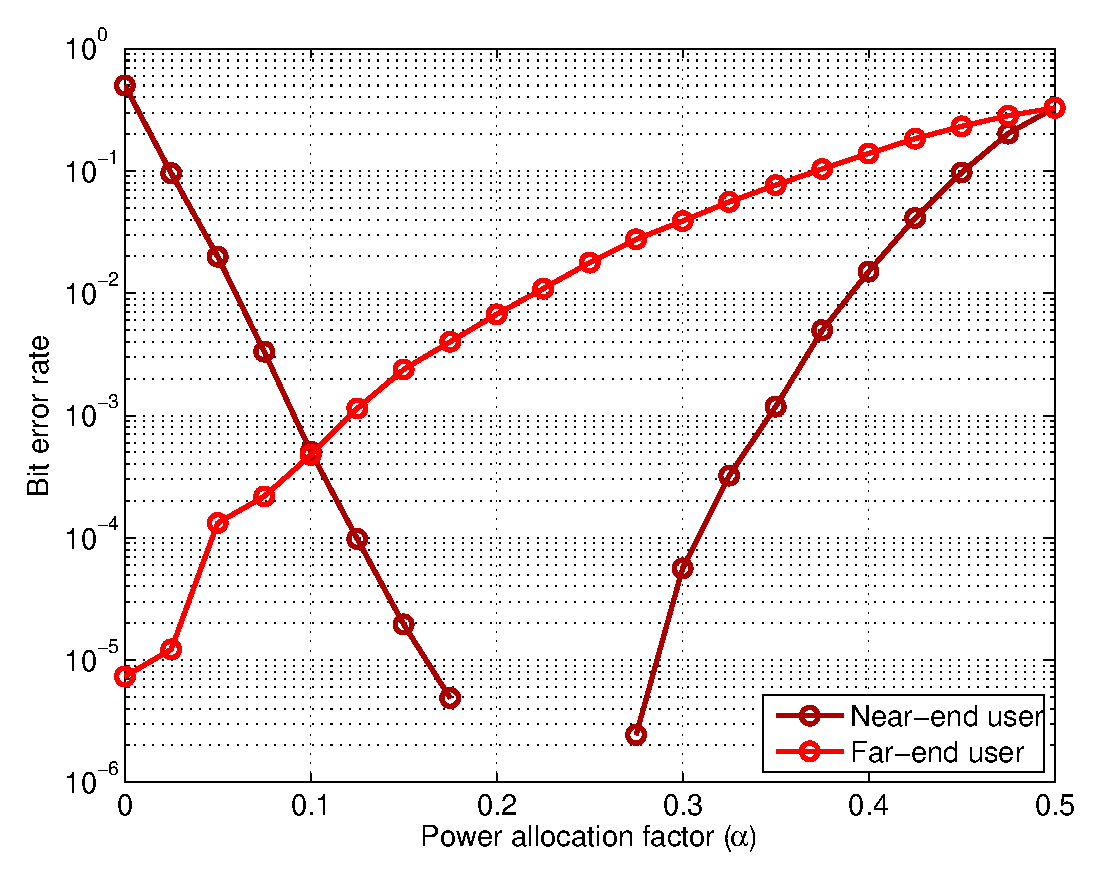
\includegraphics[width=0.95\columnwidth ,angle=0]{figure/alphaVSber.eps}
\caption{BER for different power allocation factor}
\label{fig_sim_aVSber}
\end{center}
\end{figure}
To investigate in the optimal strategy of power allocation, i.e. optimal $\alpha$
value, when serving two users.
In Fig.~\ref{fig_sim_aVSber} shows the BER to different $\alpha$ settings.
The BS transmission power is set to be $5mW/MHz$, and background noise is $-144dBm$.
Near-end user, indexed as user 1, is position at a distance of $150m$, and far-end
user, user 2, is at $220m$.
The channel loss exponent is $4.5$ and thus the PL ratio is about $5.6$.
Supposed that the system requires BER no greater than $10^-2$, $\alpha$
can be set in the range between $0.06$ and $1.17$ in this case.
\subsubsection{pair selection}
\label{pair_selection}
[Todo]
%\section{Conclusion}
%\label{sec_conclusion}

%After surveying papers, we figure out that the NOMA with SIC has a little difference in their analysis. For DOCOMO, the capacity is simply represented by ideal interference cancellation as (\ref{eq_sic_shannon}). For Bell Lab, they take the modulation and PER into consideration and the simulation results show that capacity is lower than the analysis of DOCOMO. They also propose some algorithms about resource allocation and schedule by optimization algorithm and S4 algorithm.

\section{Plan for the Next Month}
\label{sec_futureWork}

In the next month, we plan to continue investigation of NOMA on physical and MAC layers to better 
equip ourselves with state-of-the-art research advances on NOMA. In addition to theoretic, ideal models
for NOMA, we also plan to investigate more closely the simulation models presented in~\cite{cite_bell1} to lay a
more solid ground for
the resource allocation and scheduling techniques to be investigated in this project.

%In the following months, we will start to analyze NOMA with SIC and create the SNR-modulation model. What's more, in order to let optimization conveniently, we will also construct an approximation equation named SNR-throughput equation to fit the model. After finishing SNR-modulation model and SNR-throughput equation, we will propose algorithms managing resource allocation and schedule and present our results by simulation. Therefore, the SNR-modulation model, SNR-throughput equation, and algorithms will jointly construct into first version's simulator. 

%\section{Research Byproduct}
%\label{sec_product}

%None.

\section{future work}
\label{future_work}
It is positive that SIC can enhance user fairness for users in
relatively bad channel condition.
Further experiment should be done to prove that scheduling is
necessary to reach better performance gain.
It's expected that scheduling users in great difference of path
loss may reach our objective.

% citations
\bibliographystyle{IEEEtran}
\bibliography{cite}

\end{document}